% ============================================================
%  Space — Unit Booklet
%  Years 7–8  |  Victorian Curriculum F–10 Version 2.0
%  Compile with: xelatex Space_Unit_Booklet_Yr7_8.tex  (twice for page refs)
%  Fonts: ./fonts/ — same folder as Forces and Bio booklets
% ============================================================
\documentclass[11pt,a4paper]{article}

% ── Fonts (compile with XeLaTeX) ─────────────────────────────────────────────
\usepackage{fontspec}
\setmainfont{Lato}[
  Path=./fonts/, Extension=.ttf, Ligatures=TeX,
  UprightFont=Lato-Regular, ItalicFont=Lato-Italic,
  BoldFont=Lato-Bold, BoldItalicFont=Lato-BoldItalic ]
\newfontfamily\headingfont{Poppins}[
  Path=./fonts/, Extension=.ttf, Ligatures=TeX,
  UprightFont=Poppins-Regular, ItalicFont=Poppins-Italic,
  BoldFont=Poppins-Bold, BoldItalicFont=Poppins-BoldItalic ]
\setlength{\headheight}{22pt}

\usepackage[protrusion=true,expansion=false]{microtype}
\usepackage[a4paper, top=2cm, bottom=2cm, left=2cm, right=2cm]{geometry}
\usepackage{xcolor}
\usepackage{tikz}
\usetikzlibrary{arrows.meta, shapes.geometric, calc, positioning,
                decorations.pathreplacing, backgrounds, patterns}
\usepackage{tcolorbox}
\tcbuselibrary{skins, breakable, raster}
\usepackage{fancyhdr}
\usepackage{titlesec}
\usepackage{enumitem}
\usepackage{booktabs}
\usepackage{tabularx}
\usepackage{array}
\usepackage{colortbl}
\usepackage{multicol}
\usepackage{amsmath}
\usepackage{needspace}
\usepackage{lastpage}
\usepackage{calc}
\usepackage{mdframed}
\usepackage{setspace}
\usepackage{ragged2e}
\usepackage{graphicx}
\usepackage{hyperref}

% ── Colour Palette ───────────────────────────────────────────────────────────
% Primary: Space / Navy (unit identity)
\definecolor{Navy}       {HTML}{0B1A3E}
\definecolor{Space}      {HTML}{1B3378}
\definecolor{SpaceLight} {HTML}{E4E9F7}
\definecolor{SpaceMid}   {HTML}{2E4FAF}
% Gold accent
\definecolor{Gold}       {HTML}{D4A017}
\definecolor{GoldLight}  {HTML}{FBF3D5}
\definecolor{GoldDark}   {HTML}{C77F12}
% Supporting accents
\definecolor{Teal}       {HTML}{18A999}
\definecolor{TealLight}  {HTML}{E0F5F3}
\definecolor{Coral}      {HTML}{E8603C}
\definecolor{CoralLight} {HTML}{FDEEE9}
\definecolor{Violet}     {HTML}{7C4DBC}
\definecolor{VioletLight}{HTML}{F0EBF9}
% Earth / First Nations
\definecolor{Earth}      {HTML}{8B6340}
\definecolor{EarthDark}  {HTML}{5E3A1A}
\definecolor{EarthLight} {HTML}{F5EDE4}
% Neutrals
\definecolor{Ink}        {HTML}{16223A}
\definecolor{DarkGrey}   {HTML}{3A4759}
\definecolor{Grey}       {HTML}{5B6B82}   % secondary neutral; kept for body compatibility
\definecolor{MidGrey}    {HTML}{AEBED4}
\definecolor{LightGrey}  {HTML}{F2F5FA}
\definecolor{Line}       {HTML}{DDE5F0}
\definecolor{Paper}      {HTML}{FBFCFE}
% Table colours (Space-themed)
\definecolor{TableHead}  {HTML}{1B3378}
\definecolor{RowAlt}     {HTML}{E4E9F7}

% ── Hyperref ─────────────────────────────────────────────────────────────────
\hypersetup{
  colorlinks = true,
  linkcolor  = Space,
  urlcolor   = Teal,
  pdftitle   = {Space Unit Booklet --- Year 7/8 Science},
  pdfauthor  = {Northcote High School Science Department}
}

% ── Page Style ───────────────────────────────────────────────────────────────
\pagestyle{fancy}
\fancyhf{}
\renewcommand{\headrulewidth}{0.4pt}
\renewcommand{\headrule}{\hbox to\headwidth{\color{Space}\leaders\hrule height \headrulewidth\hfill}}
\fancyhead[L]{\headingfont\small\color{Space}Space}
\fancyhead[R]{\headingfont\small\color{DarkGrey}Years 7--8 \textbar{} Victorian Curriculum F--10 v2.0}
\fancyfoot[C]{\headingfont\small\color{DarkGrey}\thepage\ \textbar{} \pageref{LastPage}}
\fancypagestyle{plain}{%
  \fancyhf{}
  \fancyfoot[C]{\headingfont\small\color{DarkGrey}\thepage\ \textbar{} \pageref{LastPage}}
  \renewcommand{\headrulewidth}{0pt}
}

% ── Section Formatting ───────────────────────────────────────────────────────
\titleformat{\section}
  {\headingfont\color{Space}\Large\bfseries}
  {}{0em}{}
  [{\color{Teal}\rule[0.6ex]{2.2em}{3pt}}{\color{Line}\rule[0.6ex]{\dimexpr\linewidth-2.2em\relax}{1pt}}]
\titlespacing{\section}{0pt}{18pt}{8pt}

\titleformat{\subsection}
  {\headingfont\color{SpaceMid}\large\bfseries}
  {\thesubsection}{0.6em}{}
\titlespacing{\subsection}{0pt}{12pt}{4pt}

\titleformat{\subsubsection}
  {\headingfont\color{Space}\normalsize\bfseries}
  {}{0em}{}
\titlespacing{\subsubsection}{0pt}{8pt}{2pt}

% Deck-style eyebrow / kicker
\newcommand{\kicker}[2][Teal]{%
  {\headingfont\bfseries\footnotesize\color{#1}%
   \textcolor{#1}{\rule[0.18ex]{1.6em}{2.2pt}}\hspace{0.5em}\MakeUppercase{#2}\par}%
  \vspace{2pt}}

% ── Custom tcolorbox Environments ────────────────────────────────────────────

% Section divider banner (navy)
\newcommand{\sectiondiv}[3]{%
  \needspace{5\baselineskip}
  \begin{tcolorbox}[
    enhanced, breakable=false, arc=3.5mm,
    colback=Navy, colframe=Navy, boxrule=0pt,
    sidebyside, sidebyside align=center,
    lefthand width=2.0cm,
    left=2mm, right=4mm, top=4mm, bottom=4mm
  ]
    \begin{center}
      {\headingfont\bfseries\color{white!35!Navy}\fontsize{50}{50}\selectfont #1}
    \end{center}
    \tcblower
    {\headingfont\bfseries\color{white}\LARGE #2}\\[3pt]
    {\itshape\color{white!75!Navy}\small #3}
  \end{tcolorbox}%
}

% Key info box (space blue)
\newtcolorbox{infobox}[1]{
  breakable, arc=2.5mm, boxrule=0.5pt,
  colback=SpaceLight, colframe=Space!40,
  fonttitle=\headingfont\bfseries, coltitle=Space,
  title={#1},
  left=4mm, right=3.5mm, top=2.5mm, bottom=2.5mm
}

% First Nations callout (earth brown)
\newtcolorbox{fnbox}[1]{
  breakable, arc=2.5mm, boxrule=0.5pt,
  colback=EarthLight, colframe=Earth!40,
  fonttitle=\headingfont\bfseries, coltitle=EarthDark,
  title={#1},
  left=4mm, right=3.5mm, top=2.5mm, bottom=2.5mm
}

% Scaffold box (gold — structured student support, matches Forces/Bio)
\newtcolorbox{scaffold}[1]{
  breakable, arc=2.5mm, boxrule=0.5pt,
  colback=GoldLight, colframe=Gold!40,
  fonttitle=\headingfont\bfseries, coltitle=GoldDark,
  title={#1},
  left=4mm, right=3.5mm, top=2.5mm, bottom=2.5mm
}

% Worked example box (white bg, gold frame — matches Forces/Bio)
\newtcolorbox{workedex}[1]{
  breakable, arc=2.5mm, boxrule=0.5pt,
  colback=white, colframe=Gold!50,
  fonttitle=\headingfont\bfseries, coltitle=GoldDark,
  title={#1},
  left=4mm, right=3.5mm, top=2.5mm, bottom=2.5mm
}

% Year 7 box (space blue)
\newtcolorbox{yr7box}{
  breakable, arc=2.5mm, boxrule=0.5pt,
  colback=SpaceLight, colframe=Space!40,
  left=4mm, right=3.5mm, top=2.5mm, bottom=2.5mm
}

% Year 8 extension box (violet — same across all units)
\newtcolorbox{yr8box}{
  breakable, arc=2.5mm, boxrule=0.5pt,
  colback=VioletLight, colframe=Violet!40,
  left=4mm, right=3.5mm, top=2.5mm, bottom=2.5mm
}

% ── Custom Commands ───────────────────────────────────────────────────────────

% Answer box: \answerbox{height e.g. 3cm}
\newcommand{\answerbox}[1]{%
  \begin{tcolorbox}[
    enhanced, breakable, arc=2mm,
    colback=Paper, colframe=Line,
    left=2mm, right=2mm, top=1mm, bottom=1mm,
    boxrule=1pt, height=#1
  ]
  \end{tcolorbox}%
}

% Question: \question{number}{marks}{text}  (marks can be empty)
\newcommand{\question}[3]{%
  \needspace{3\baselineskip}%
  \medskip
  \noindent\textbf{Q#1}\ifx&#2&\else\ \textcolor{DarkGrey}{(#2 mark\ifnum#2=1\else s\fi)}\fi\quad #3%
  \medskip
}

% Inline marks note
\newcommand{\markscount}[1]{\hfill\textcolor{DarkGrey}{\textit{(#1 mark\ifnum#1=1\else s\fi)}}}

% Figure caption
\newcommand{\figcap}[1]{%
  \begin{center}\small\itshape\color{DarkGrey} #1\end{center}%
}

% Answer lines: \anslines{n}
\newcommand{\anslines}[1]{%
  \vspace{2pt}%
  \foreach \n in {1,...,#1}{%
    \par\noindent\rule{\linewidth}{0.3pt}\vspace{3pt}%
  }%
}

% Table column types
\newcolumntype{L}[1]{>{\RaggedRight\arraybackslash}p{#1}}
\newcolumntype{C}[1]{>{\Centering\arraybackslash}p{#1}}

% Table helpers
\newcommand{\thead}[1]{\cellcolor{TableHead}\color{white}\bfseries #1}
\newcommand{\talt}{\rowcolor{RowAlt}}
\newcommand{\tmid}{\rowcolor{MidGrey}}

% Vocabulary term
\newcommand{\vocab}[1]{\textbf{\textcolor{Space}{#1}}}

% Victorian Curriculum reference
\newcommand{\vc}[2]{\small\textcolor{DarkGrey}{\textit{VC 2.0: #1 --- #2}}}


% ============================================================
\begin{document}
% ============================================================

% ---- TITLE PAGE --------------------------------------------
\begin{titlepage}
\pagecolor{Navy}
\color{white}
\vspace*{3cm}
\begin{center}
  {\headingfont\fontsize{11pt}{13pt}\selectfont\color{Gold}
    NORTHCOTE HIGH SCHOOL\ \textbullet\ YEAR 7/8 SCIENCE\ \textbullet\ VICTORIAN CURRICULUM 2.0}

  \vspace{1.4cm}
  {\headingfont\fontsize{42pt}{46pt}\selectfont\bfseries Space}

  \vspace{0.8cm}
  {\headingfont\fontsize{18pt}{22pt}\selectfont\color{SpaceLight}
    Student Workbook}

  \vspace{2.2cm}
  \textcolor{Gold}{\rule{10cm}{1.5pt}}

  \vspace{1.8cm}
  {\fontsize{12pt}{16pt}\selectfont\color{SpaceLight}
    Covering 11 lessons across Sections 1--11:}

  \vspace{0.6cm}
  {\fontsize{11pt}{15pt}\selectfont\color{white!85!Navy}
    Earth, Moon \& Sun \textbullet\ Day, Night \& Seasons \textbullet\ Moon Phases \& Tides\\[0.3em]
    Our Solar System \textbullet\ Stars \& Galaxies \textbullet\ Space Exploration\\[0.3em]
    Gravity \& Orbits \textbullet\ Light \& Telescopes \textbullet\ Aboriginal Astronomy\\[0.3em]
    Space \& Sustainability \textbullet\ The Search for Life}

  \vspace{2.4cm}
  \textcolor{Gold}{\rule{10cm}{1.5pt}}

  \vspace{1.6cm}
  {\fontsize{11pt}{14pt}\selectfont\color{SpaceLight}
    Name: \underline{\hspace{7cm}}\ \ \ Class: \underline{\hspace{3cm}}}

  \vspace{0.6cm}
  {\fontsize{10pt}{13pt}\selectfont\color{white!60!Navy}
    \textit{We acknowledge the Wurundjeri-Woiwurrung people of the Kulin Nation\\
    as the Traditional Custodians of the Country on which we learn.}}
\end{center}
\end{titlepage}

\nopagecolor
\newpage

% ---- ACKNOWLEDGEMENT OF COUNTRY ----------------------------
\begin{fnbox}{Acknowledgement of Country}
We acknowledge the Wurundjeri-Woiwurrung people of the Kulin Nation as the Traditional Custodians of the Country on which Northcote High School stands. We pay our respects to Elders past, present, and emerging. Aboriginal and Torres Strait Islander astronomical knowledge --- developed over tens of thousands of years --- is woven throughout this unit as living, ongoing science, not as a historical artefact.

\medskip
\textit{Throughout this booklet, the} \textcolor{Earth}{\textbf{earth-coloured boxes}} \textit{highlight First Nations perspectives and knowledge. These are integral to the science we study, not supplementary.}
\end{fnbox}

\vspace{0.5em}

\begin{infobox}{How to use this booklet}
\begin{itemize}
  \item This booklet accompanies all 11 lessons of the Space unit
  \item Work through each section during class; complete starred questions ($\star$) for homework
  \item \textbf{Year 7} students complete all unshaded sections
  \item \textbf{Year 8} students also complete the \textcolor{Violet}{\textbf{purple Year 8 Extension}} boxes in each section
  \item Diagrams and tables with blank spaces are for you to complete during the lesson
  \item Vocabulary terms are shown in \vocab{bold blue} --- add them to your glossary
\end{itemize}
\end{infobox}

\tableofcontents
\newpage

% ============================================================
\section{Earth, Moon and Sun --- Scale and Structure}
% ============================================================
\vc{Science Understanding}{Physical sciences: Earth and space sciences; scale and relative size of Earth, Moon and Sun}

\subsection{The scale of Earth, Moon and Sun}

The three most important objects in our immediate cosmic environment differ enormously in size. Understanding their relative sizes is foundational to everything else in this unit.

\begin{center}
\begin{tabular}{lrrr}
\toprule
\headingfont\textbf{Object} & \headingfont\textbf{Diameter (km)} & \headingfont\textbf{Mass (kg)} & \headingfont\textbf{Distance from Earth} \\
\midrule
Moon    & 3,474          & $7.34\times10^{22}$  & 384,400 km avg \\
Earth   & 12,742         & $5.97\times10^{24}$  & ---             \\
Sun     & 1,392,000      & $1.99\times10^{30}$  & 150,000,000 km (1 AU) \\
\bottomrule
\end{tabular}
\end{center}

\begin{infobox}{Key concept: Scale}
If Earth were the size of a tennis ball (6.7 cm across), the Moon would be a marble (1.8 cm) about 1.9 m away, and the Sun would be a sphere 7.5 m across, placed 807 m down the road. The solar system is almost entirely \vocab{empty space}.
\end{infobox}

\subsection{Structure of Earth}

Earth has four main layers:
\begin{itemize}
  \item \vocab{Inner core} --- solid iron-nickel; radius ~1,200 km; temperature ~5,400°C
  \item \vocab{Outer core} --- liquid iron-nickel; generates Earth's magnetic field (the dynamo effect)
  \item \vocab{Mantle} --- semi-solid rock; 2,900 km thick; convection currents drive plate tectonics
  \item \vocab{Crust} --- thin, solid rock; 5--70 km thick; oceanic (denser, thinner) and continental (less dense, thicker)
\end{itemize}

\subsubsection{Diagram: Label the layers of Earth}
\begin{center}
\begin{tikzpicture}
  \fill[color=Space!80]        (0,0) circle (3.6cm);
  \fill[color=Space!50]        (0,0) circle (2.8cm);
  \fill[color=Space!30]        (0,0) circle (1.5cm);
  \fill[color=Gold!70]         (0,0) circle (0.7cm);
  % Label lines
  \draw[Grey, ->] (0.7,0)   -- (1.1,0.6)  node[right, font=\small] {Inner core};
  \draw[Grey, ->] (1.1,0)   -- (1.6,0.9)  node[right, font=\small] {Outer core};
  \draw[Grey, ->] (1.8,0)   -- (2.4,1.2)  node[right, font=\small] {Mantle};
  \draw[Grey, ->] (2.9,0.2) -- (3.4,1.4)  node[right, font=\small] {Crust};
\end{tikzpicture}
\end{center}

\subsection{Structure of the Sun}

The Sun is a \vocab{main sequence star} --- it converts hydrogen into helium through \vocab{nuclear fusion} in its core.

\begin{itemize}
  \item \textbf{Core}: where fusion occurs; temperature ~15 million°C
  \item \textbf{Radiative zone}: energy moves outward as photons (takes ~100,000 years to cross)
  \item \textbf{Convective zone}: energy carried by convecting plasma
  \item \textbf{Photosphere}: the visible surface (~5,778 K); where sunspots form
  \item \textbf{Chromosphere and Corona}: outer atmosphere; much hotter than photosphere (corona: 1--3 million K)
\end{itemize}

\begin{fnbox}{Boorong sky knowledge: the Sun and warmth}
For the Boorong people of north-western Victoria, the Sun (\textit{Gnowee}) is an ancestral woman who carries a torch across the sky each day. This narrative encodes the observable fact of solar motion and the Sun's role as the source of warmth and light. The daily and seasonal variation in the Sun's position --- which the Boorong tracked with precision --- reflects the same gravitational physics that determines Earth's seasons.
\end{fnbox}

\begin{workedex}{Worked example: Light travel time from the Sun}
\textit{The Sun is 150,000,000 km from Earth. Light travels at 300,000 km/s. How long does sunlight take to reach us?}

\medskip
$\text{Time} = \dfrac{\text{Distance}}{\text{Speed}} = \dfrac{150{,}000{,}000 \text{ km}}{300{,}000 \text{ km/s}} = 500 \text{ s} = 8 \text{ min } 20 \text{ s}$

\medskip
\textbf{Answer}: Sunlight takes 8 minutes and 20 seconds to reach Earth. This means the Sun we see right now is actually how it looked 8 minutes ago.
\end{workedex}

\begin{scaffold}{Your turn: Q1.1}
A flash of light leaves the Moon. How long before we see it? (Moon is 384,400 km away; speed of light = 300,000 km/s)

\vspace{2.5cm}
\end{scaffold}

\newpage
% ============================================================
\section{Day, Night and Seasons}
% ============================================================
\vc{Science Understanding}{Earth and space sciences: Earth's rotation and revolution; axial tilt and seasons}

\subsection{Why we have day and night}

Earth \vocab{rotates} (spins on its axis) once every \textbf{24 hours}. The side facing the Sun experiences day; the opposite side experiences night.

\begin{itemize}
  \item Earth rotates \vocab{west to east} (anticlockwise when viewed from above the North Pole)
  \item This is why the Sun appears to rise in the east and set in the west
  \item Earth also \vocab{revolves} (orbits) around the Sun once every 365.25 days --- one year
\end{itemize}

\subsection{Why we have seasons}

Seasons are caused by Earth's \vocab{axial tilt} of 23.5°, not by distance from the Sun. (Earth is actually closest to the Sun in January --- Australian summer.)

\begin{infobox}{Why tilt causes seasons}
When the Southern Hemisphere tilts toward the Sun (December):
\begin{itemize}
  \item The Sun is higher in the sky --- its rays hit at a more direct angle (more energy per m$^2$)
  \item Days are longer --- more hours of sunlight
  \item The combination produces \textbf{summer} in Australia
\end{itemize}
When the Southern Hemisphere tilts away (June): rays hit at a shallower angle, days are shorter --- \textbf{winter}.
\end{infobox}

\subsection{Solstices and equinoxes}

\begin{center}
\begin{tabular}{lll}
\toprule
\textbf{Event} & \textbf{Date (approx.)} & \textbf{What happens} \\
\midrule
December solstice & 21--22 December & Southern Hemisphere longest day; summer solstice for Australia \\
June solstice     & 21--22 June     & Southern Hemisphere shortest day; winter solstice for Australia \\
March equinox     & 20--21 March    & Equal day/night worldwide; autumn begins in Australia \\
September equinox & 22--23 September& Equal day/night worldwide; spring begins in Australia \\
\bottomrule
\end{tabular}
\end{center}

\begin{fnbox}{Wurundjeri six-season calendar}
The Wurundjeri-Woiwurrung people recognise \textbf{six seasons} on Kulin Nation Country, each defined by ecological signals and celestial indicators rather than fixed calendar dates. The transitions are marked by changes in animal behaviour, plant flowering, rainfall patterns, and the position of stars and the Milky Way. This is a more ecologically precise calendar than the European four-season model for this Country.

\medskip
\begin{tabular}{ll}
\textit{Iuk} (eel season) & Autumn rains, eels run \\
\textit{Waring} & Winter cold, least food \\
\textit{Guling} & Orchids bloom, first warmth \\
\textit{Poorneet} & Tadpole season, frogs call \\
\textit{Buath Gurru} & Grasshoppers swarm \\
\textit{Kangaroo Apple season} & Fruit ripens, late summer \\
\end{tabular}
\end{fnbox}

\begin{scaffold}{Your turn: Q2.1}
Explain why Australia has summer in December while countries in the Northern Hemisphere have winter at the same time. Use the concept of axial tilt in your answer.

\vspace{3.5cm}
\end{scaffold}

\newpage
% ============================================================
\section{The Moon --- Phases and Tides}
% ============================================================
\vc{Science Understanding}{Earth and space sciences: Moon phases and tidal patterns; gravitational effects}

\subsection{Why the Moon appears to change shape}

The Moon does not produce light --- it \vocab{reflects sunlight}. At all times, the half facing the Sun is lit. As the Moon orbits Earth over \textbf{29.5 days}, we see different fractions of the lit half from Earth --- these are the \vocab{phases}.

\begin{infobox}{Common misconception}
Earth's shadow does \textbf{NOT} cause phases. A \vocab{lunar eclipse} (Earth's shadow on the Moon) is a separate, less frequent event. Phases are caused by our changing view of the Moon's lit half.
\end{infobox}

\subsubsection{The eight phases (in order)}
New Moon $\rightarrow$ Waxing crescent $\rightarrow$ First quarter $\rightarrow$ Waxing gibbous $\rightarrow$ Full Moon $\rightarrow$ Waning gibbous $\rightarrow$ Third quarter $\rightarrow$ Waning crescent $\rightarrow$ New Moon

\subsection{Tides}

The Moon's gravity pulls on Earth's oceans. This creates a \vocab{tidal bulge} on the Moon-facing side, and a second bulge on the opposite side.

\begin{itemize}
  \item \vocab{Spring tides}: Sun, Earth, and Moon are aligned (new or full Moon). Gravitational pulls add together --- very large tidal range
  \item \vocab{Neap tides}: Moon at right angles to the Sun--Earth line (quarter phases). Pulls partially cancel --- moderate tidal range
  \item ``Spring'' refers to the Old English word for ``to leap,'' not the season
\end{itemize}

\begin{fnbox}{Lunar calendars in Aboriginal traditions}
Many Aboriginal Australian groups have used the 29.5-day lunar cycle for ceremony, food harvesting, travel, and health practices. For Kulin Nation groups, the monthly cycle is embedded in governance and knowledge transmission. The same lunar cycle that determines tides was used to create a precise, multi-purpose calendar operating on Country long before European contact.
\end{fnbox}

\begin{yr8box}
\textbf{Year 8 Extension: Eclipse geometry}

Eclipses don't happen every New or Full Moon because the Moon's orbit is tilted 5.1° relative to Earth's orbit around the Sun. Eclipses only occur when a New or Full Moon coincides with the Moon being at a \vocab{node} (one of two points where its orbit crosses the ecliptic). The pattern of eclipses repeats every 18 years, 11 days, 8 hours --- the \vocab{Saros cycle}.

\medskip
\textbf{Why the Moon fits the Sun perfectly}: The Moon is 400$\times$ smaller than the Sun but 400$\times$ closer. Their angular diameters in our sky are almost identical --- making total solar eclipses possible. This is unique in our solar system.
\end{yr8box}

\newpage
% ============================================================
\section{Our Solar System}
% ============================================================
\vc{Science Understanding}{Earth and space sciences: Structure and scale of the solar system; classification of planets}

\subsection{The eight planets}

\begin{center}
\begin{tabular}{llrrl}
\toprule
\textbf{Planet} & \textbf{Type} & \textbf{Distance (AU)} & \textbf{Diameter (km)} & \textbf{Moons} \\
\midrule
Mercury & Terrestrial & 0.39  & 4,879     & 0   \\
Venus   & Terrestrial & 0.72  & 12,104    & 0   \\
Earth   & Terrestrial & 1.00  & 12,742    & 1   \\
Mars    & Terrestrial & 1.52  & 6,779     & 2   \\
Jupiter & Gas giant   & 5.20  & 139,820   & 95  \\
Saturn  & Gas giant   & 9.54  & 116,460   & 146 \\
Uranus  & Ice giant   & 19.2  & 50,724    & 28  \\
Neptune & Ice giant   & 30.1  & 49,244    & 16  \\
\bottomrule
\end{tabular}
\end{center}

Mnemonic: \textbf{M}y \textbf{V}ery \textbf{E}xcited \textbf{M}other \textbf{J}ust \textbf{S}erved \textbf{U}s \textbf{N}oodles

\begin{infobox}{What is an Astronomical Unit (AU)?}
1 \vocab{AU} = the average Earth--Sun distance = approximately 150,000,000 km. This unit makes solar system distances much easier to write and compare. Neptune is 30 AU from the Sun --- thirty times farther from the Sun than Earth.
\end{infobox}

\subsection{Other solar system objects}

\begin{itemize}
  \item \vocab{Asteroid belt}: between Mars and Jupiter; rocky/metallic objects; gravitational influence of Jupiter prevented these from forming a planet
  \item \vocab{Dwarf planets}: Pluto, Ceres, Eris, Haumea, Makemake --- too small and haven't cleared their orbital neighbourhood
  \item \vocab{Kuiper Belt}: beyond Neptune (30--50 AU); icy objects including Pluto
  \item \vocab{Comets}: icy bodies; develop a tail of gas and dust when they approach the Sun
  \item \vocab{Oort Cloud}: distant spherical shell of icy objects; source of long-period comets
\end{itemize}

\begin{fnbox}{The Emu in the Sky and planet tracking}
The Boorong people of Victoria observed and named the five naked-eye planets --- Mercury, Venus, Mars, Jupiter, and Saturn --- tracking their movements over decades and centuries. The dark dust lanes of the Milky Way, traced as the \textbf{Emu in the Sky}, provided a backdrop against which planetary motion was measured. The Emu's seasonal position and orientation also indicates when emus are laying eggs --- a verified ecological calendar encoded in sky observation.
\end{fnbox}

\begin{workedex}{Worked example: Travel time using AU}
\textit{Saturn is 9.5 AU from the Sun. Earth is 1 AU, so the Earth--Saturn distance is approximately 8.5 AU. At 60,000 km/h, how long does the trip take?}

$8.5 \times 150{,}000{,}000 = 1{,}275{,}000{,}000 \text{ km}$

$\text{Time} = \frac{1{,}275{,}000{,}000}{60{,}000} = 21{,}250 \text{ hours} = 885 \text{ days} \approx \mathbf{2.4 \text{ years}}$
\end{workedex}

\begin{yr8box}
\textbf{Year 8 Extension: Kepler's Laws of Planetary Motion}

Johannes Kepler derived three laws from careful observation of planetary data:
\begin{enumerate}
  \item \textbf{Law of Ellipses}: Planets orbit the Sun in ellipses, with the Sun at one focus.
  \item \textbf{Law of Equal Areas}: A planet sweeps equal areas in equal times --- moves faster when closer to the Sun.
  \item \textbf{Harmonic Law}: $T^2 \propto a^3$ --- orbital period squared is proportional to semi-major axis cubed.
\end{enumerate}
\textbf{Apply Law 3}: Mars is 1.52 AU from the Sun. Orbital period: $T = 1.52^{3/2} \approx 1.87$ years (687 Earth days).
\end{yr8box}

\newpage
% ============================================================
\section{Beyond the Solar System --- Stars and Galaxies}
% ============================================================
\vc{Science Understanding}{Earth and space sciences: Properties of stars; galaxies; scale of the universe}

\subsection{Light-years and stellar distances}

A \vocab{light-year} is the distance light travels in one year: approximately $9.46 \times 10^{12}$ km (9.46 trillion km). It is a unit of \textit{distance}, not time.

\begin{itemize}
  \item The Sun: light takes 8 min 20 s to reach Earth
  \item Proxima Centauri (nearest star): 4.2 light-years
  \item Milky Way diameter: $\approx$100,000 light-years
  \item Andromeda Galaxy: 2.5 million light-years
\end{itemize}

\begin{infobox}{Looking back in time}
When we observe a star 100 light-years away, we see it as it was 100 years ago --- the light we detect left it then. Telescopes are time machines. JWST images galaxies as they appeared just 300--400 million years after the Big Bang.
\end{infobox}

\subsection{Star types and the OBAFGKM sequence}

Stars are classified by surface temperature and colour:

\begin{center}
\begin{tabular}{lllr}
\toprule
\textbf{Class} & \textbf{Colour} & \textbf{Temperature} & \textbf{Example} \\
\midrule
O & Blue-violet & $>$30,000 K & Zeta Puppis \\
B & Blue-white  & 10,000--30,000 K & Rigel \\
A & White       & 7,500--10,000 K & Sirius \\
F & Yellow-white& 6,000--7,500 K & Procyon \\
G & Yellow      & 5,200--6,000 K & \textbf{The Sun} \\
K & Orange      & 3,700--5,200 K & Arcturus \\
M & Red         & $<$3,700 K & Proxima Centauri \\
\bottomrule
\end{tabular}
\end{center}

\subsection{Stellar life cycle (sun-like star)}

\begin{center}
\begin{tikzpicture}[node distance=1.4cm, >=Stealth]
  \node[draw=Space!40, rounded corners=3pt, fill=SpaceLight, font=\small, minimum width=1.8cm, minimum height=0.7cm] (neb) {Nebula};
  \node[draw=Space!40, rounded corners=3pt, fill=SpaceLight, font=\small, minimum width=1.8cm, minimum height=0.7cm, right=of neb] (pro) {Protostar};
  \node[draw=Gold!50, rounded corners=3pt, fill=GoldLight, font=\small, minimum width=2cm, minimum height=0.7cm, right=of pro] (ms) {\textbf{Main seq.}};
  \node[draw=Coral!40, rounded corners=3pt, fill=CoralLight, font=\small, minimum width=2cm, minimum height=0.7cm, right=of ms] (rg) {Red giant};
  \node[draw=Space!40, rounded corners=3pt, fill=SpaceLight, font=\small, minimum width=2cm, minimum height=0.7cm, right=of rg] (wd) {White dwarf};
  \draw[->] (neb) -- (pro);
  \draw[->] (pro) -- (ms);
  \draw[->] (ms) -- (rg);
  \draw[->] (rg) -- (wd);
\end{tikzpicture}

\vspace{0.4em}
\small\textit{Massive stars ($>$8 M$_\odot$): Main sequence $\rightarrow$ Red supergiant $\rightarrow$ Supernova $\rightarrow$ Neutron star / Black hole}
\end{center}

\begin{fnbox}{Boorong knowledge: The Magellanic Clouds}
The Large and Small Magellanic Clouds --- dwarf galaxies visible to the naked eye from the Southern Hemisphere --- are incorporated into Boorong star lore as \textit{Yugarilya}, the two Bram-bram-bult (sons of Bunjil the creator), who appear as wedge-tailed eagles in the sky. Aboriginal Australians observed these objects for tens of thousands of years before European astronomers named them after Magellan's 1521 voyage.
\end{fnbox}

\begin{yr8box}
\textbf{Year 8 Extension: The Hertzsprung--Russell Diagram}

The H--R diagram plots stellar luminosity (vertical axis) against surface temperature (horizontal axis, running \textit{right to left} --- hot on left). Stars cluster in recognisable zones: the \vocab{main sequence} (a diagonal band), the \vocab{giant branch} (upper right, cool but luminous), and \vocab{white dwarfs} (lower left, hot but dim). A star's position reveals its evolutionary stage, mass, and age.
\end{yr8box}

\newpage
% ============================================================
\section{Space Exploration --- History and Technology}
% ============================================================
\vc{Science Understanding}{Science as a Human Endeavour: Space exploration technologies; Australian contributions}

\subsection{Key milestones in space exploration}

\begin{center}
\begin{tabular}{rll}
\toprule
\textbf{Year} & \textbf{Event} & \textbf{Significance} \\
\midrule
1957 & Sputnik 1 (USSR) & First artificial satellite \\
1961 & Yuri Gagarin (USSR) & First human in orbit \\
1969 & Apollo 11 (USA) & First humans on the Moon \\
1990 & Hubble Space Telescope & Revolutionised optical astronomy \\
1998 & ISS construction begins & First permanent human presence in space \\
2012 & Curiosity rover lands on Mars & Searches for habitability \\
2021 & JWST launched & Infrared view of the early universe \\
2024 & Europa Clipper launched & Searching for habitability on Europa \\
\bottomrule
\end{tabular}
\end{center}

\subsection{Australia's contributions to space science}

\begin{itemize}
  \item \textbf{Parkes Radio Telescope} (``The Dish'') --- received and relayed live TV of the Apollo 11 Moon landing to 600 million viewers worldwide (1969)
  \item \textbf{CSIRO} --- invented Wi-Fi technology from radio astronomy research; operates major Australian telescope networks
  \item \textbf{Australian Space Agency (ASA)} --- established 2018; growing commercial space sector targeting A\$12 billion by 2030
  \item \textbf{Square Kilometre Array (SKA)} --- world's largest radio telescope, core in WA on Wajarri Country
\end{itemize}

\begin{fnbox}{Wajarri Yamatji Country and the SKA}
The Square Kilometre Array is being built on \textbf{Wajarri Yamatji Country} in the Murchison region of Western Australia --- chosen for its radio-quiet environment and extraordinarily dark skies. The Wajarri Yamatji have a formal Indigenous Land Use Agreement with the Australian government, including veto rights and community benefit provisions. The Wajarri people have maintained detailed sky knowledge of this Country for tens of thousands of years. The SKA is a model of how Western science can operate in genuine partnership with Traditional Custodians.
\end{fnbox}

\begin{scaffold}{Your turn: Q6.1 --- Mission evaluation}
Choose one of the following and evaluate it as a scientific mission. State: (a) the goal; (b) whether it was crewed or uncrewed and why; (c) one key discovery; (d) one limitation.

\medskip
\textit{Options: Apollo 11, Hubble Space Telescope, Curiosity rover, JWST}

\vspace{5cm}
\end{scaffold}

\newpage
% ============================================================
\section{Gravity and Orbits}
% ============================================================
\vc{Science Understanding}{Physical sciences: Gravitational force; orbital motion; Newton's law of universal gravitation}

\subsection{Newton's law of universal gravitation}

Every object with mass attracts every other object with mass:

\begin{center}
\Large $F = \dfrac{G \cdot m_1 \cdot m_2}{r^2}$
\end{center}

Where: $F$ = gravitational force (N), $G$ = gravitational constant ($6.67 \times 10^{-11}$ N\,m$^2$/kg$^2$), $m_1, m_2$ = masses (kg), $r$ = distance between centres (m).

\begin{itemize}
  \item Double either mass $\rightarrow$ force doubles
  \item Double the distance $\rightarrow$ force decreases to \textbf{one quarter} (inverse square law)
  \item Gravity is always \textit{attractive} --- it only pulls, never pushes
\end{itemize}

\subsection{Orbital motion}

An \vocab{orbit} occurs when gravity provides the centripetal force needed to keep an object moving in a curved path. Orbiting objects are in constant \vocab{free fall} toward the body they orbit --- but moving forward so fast they keep missing it.

\begin{infobox}{Why astronauts appear weightless}
The ISS orbits at $\approx$408 km altitude, where gravity is about 90\% of surface strength. Astronauts appear weightless because they \textit{and} the station are falling together at the same rate. ``Weightlessness'' is free fall --- not absence of gravity.
\end{infobox}

\subsection{Orbital speed and altitude}

Higher altitude = lower orbital speed (and longer period):

\begin{center}
\begin{tabular}{llrr}
\toprule
\textbf{Orbit} & \textbf{Altitude} & \textbf{Speed} & \textbf{Period} \\
\midrule
LEO (ISS) & 200--2,000 km & $\approx$7.9 km/s & $\approx$90 min \\
MEO (GPS) & 2,000--35,786 km & $\approx$3.9 km/s & $\approx$12 h \\
GEO (comms, weather) & 35,786 km & $\approx$3.1 km/s & 24 h \\
\bottomrule
\end{tabular}
\end{center}

\begin{fnbox}{Celestial navigation on Wurundjeri Country}
The predictability of orbital motion --- every star rises at a known azimuth, every planet follows a known path --- is what makes celestial navigation possible. The Wurundjeri-Woiwurrung used the Southern Cross, the Two Pointers (Alpha and Beta Centauri), and the seasonal movement of the Milky Way to navigate across Country with precision. This is applied orbital mechanics, developed through systematic observation over tens of thousands of years.
\end{fnbox}

\begin{workedex}{Worked example: Weight at ISS altitude}
\textit{An astronaut weighs 700 N on Earth (radius 6,371 km). What is their weight at ISS altitude (408 km above surface)?}

$r_\text{ISS} = 6{,}371 + 408 = 6{,}779$ km

Force ratio $= \left(\dfrac{6{,}371}{6{,}779}\right)^2 = 0.883$

Weight at ISS $= 700 \times 0.883 = \mathbf{618 \text{ N}}$ (about 88\% of surface weight)
\end{workedex}

\begin{yr8box}
\textbf{Year 8 Extension: Escape velocity}

To escape a planet's gravitational field entirely: $v_e = \sqrt{\dfrac{2GM}{r}}$

Earth: 11.2 km/s \quad Moon: 2.4 km/s \quad Mars: 5.0 km/s \quad Jupiter: 59.5 km/s

The Moon's low escape velocity explains why it has no atmosphere: gas molecules moving at thermal speeds can escape to space over time.
\end{yr8box}

\newpage
% ============================================================
\section{Light from Space --- Telescopes and the EM Spectrum}
% ============================================================
\vc{Science Understanding}{Physical sciences: Electromagnetic radiation; wave properties; telescopes as scientific instruments}

\subsection{The electromagnetic spectrum}

Visible light is only a small part of the \vocab{electromagnetic spectrum} (EM spectrum). All EM waves travel at the speed of light ($3 \times 10^8$ m/s) but differ in wavelength and frequency.

\begin{center}
\begin{tabular}{lllp{5cm}}
\toprule
\textbf{Region} & \textbf{Wavelength} & \textbf{Energy} & \textbf{Astronomical use} \\
\midrule
Radio waves  & mm to km   & Lowest  & Pulsars, CMB, galaxy mapping (Parkes, SKA) \\
Microwaves   & mm         & Low     & CMB, molecular clouds \\
Infrared     & 1\,$\mu$m--1\,mm & Medium-low & Star formation, cool objects, exoplanet atmospheres (JWST) \\
Visible      & 400--700 nm & Medium & Stars, planets, galaxies (optical telescopes) \\
UV           & 10--400 nm  & Medium-high & Hot stars, quasars \\
X-ray        & 0.01--10 nm & High   & Black holes, neutron stars, galaxy clusters \\
Gamma ray    & $<$0.01 nm & Highest & Supernovae, gamma-ray bursts \\
\bottomrule
\end{tabular}
\end{center}

\subsection{Telescopes}

\begin{itemize}
  \item \vocab{Refracting telescopes}: glass lenses bend light to a focus. Limited to small instruments
  \item \vocab{Reflecting telescopes}: mirrors reflect light to a focus. All major modern telescopes; can be built much larger (Hubble: 2.4 m mirror; JWST: 6.5 m)
  \item \vocab{Radio telescopes}: large dish antennas; collect radio waves; Parkes dish (64 m) relayed Moon landing footage
  \item \vocab{Space telescopes}: above the atmosphere; avoid absorption and blurring; JWST orbits at the Sun--Earth L2 point
\end{itemize}

\subsection{Spectroscopy --- reading starlight}

When starlight passes through a prism or diffraction grating, \vocab{absorption lines} appear --- dark lines at specific wavelengths absorbed by elements in the star's outer atmosphere. Each element has a unique spectral fingerprint. From absorption spectra, astronomers determine:
\begin{itemize}
  \item Elemental \vocab{composition} of stars and exoplanet atmospheres
  \item \vocab{Temperature} (line types reveal temperature class)
  \item \vocab{Velocity}: blueshifted = moving toward us; redshifted = moving away (Doppler effect)
\end{itemize}

\begin{fnbox}{Wajarri knowledge and the MWA}
The Murchison Widefield Array (MWA) --- precursor to the SKA --- sits on Wajarri Yamatji Country in Western Australia. It maps hydrogen across the Milky Way using radio waves invisible to the naked eye. The Wajarri have observed and named features of this same sky for tens of thousands of years using different instruments (their senses, memory, and song). Both the MWA and Wajarri sky knowledge reveal the same cosmos at different scales and with different tools.
\end{fnbox}

\begin{yr8box}
\textbf{Year 8 Extension: Interferometry and the Event Horizon Telescope}

By linking multiple radio telescopes worldwide and combining their signals with atomic-clock precision, astronomers create a \vocab{virtual telescope} as large as the separation between dishes --- a technique called \vocab{interferometry}. The \textbf{Event Horizon Telescope} linked 8 observatories to create an Earth-sized virtual dish, imaging the shadow of a black hole in galaxy M87 (2019) and the Milky Way's central black hole Sgr A* (2022). Resolution achieved: 40 microarcseconds --- equivalent to reading a newspaper in New York from Sydney.
\end{yr8box}

\newpage
% ============================================================
\section{Aboriginal and Torres Strait Islander Astronomy}
% ============================================================
\vc{Science Understanding}{Science as a Human Endeavour: Indigenous knowledge systems; dark constellations; ecological calendars}

\begin{fnbox}{Context: The world's oldest astronomical traditions}
Aboriginal and Torres Strait Islander peoples have practised systematic astronomy for at least 65,000 years --- making these the oldest continuing astronomical traditions on Earth. This is not historical knowledge. It is a living, ongoing science embedded in ceremony, ecology, governance, and art.
\end{fnbox}

\subsection{Dark constellations}

Western constellation traditions connect \textit{stars} into figures. Aboriginal traditions also identify figures formed by the \vocab{dark dust lanes} of the Milky Way --- regions of interstellar dust that block the light of stars behind them.

\begin{itemize}
  \item The \vocab{Emu in the Sky}: head = Coalsack Nebula (near the Southern Cross); body traces dark lanes along the Milky Way. When the Emu's head is near the horizon at dusk in autumn, emus are laying eggs --- verified independently by zoologists
  \item Other dark constellations: Possum, Caterpillar, Pregnant Woman, Wedge-tailed Eagle
  \item The dark areas are \vocab{molecular clouds} --- real, scientifically significant objects and birthplaces of new stars
\end{itemize}

\subsection{The Boorong star catalogue}

The Boorong people (Wergaia, north-western Victoria) have one of the best-documented Aboriginal astronomical knowledge systems. With the assistance of Elder William Barak, surveyor William Stanbridge documented 47 named celestial objects in 1857:

\begin{itemize}
  \item The Magellanic Clouds (as \textit{Yugarilya})
  \item Open star clusters (Pleiades, Hyades)
  \item Variable stars
  \item A record of the Eta Carinae brightening event of c.1843 (\textit{Collowgulloric War}) --- consistent with European records of the same event
\end{itemize}

\subsection{The sky as ecological calendar}

\begin{fnbox}{Wurundjeri sky knowledge in practice}
On Wurundjeri Country, the rising of the Pleiades (Seven Sisters, \textit{Nurrumbunguttias}) marks the transition between seasons and signals specific ecological activities. The six-season Kulin calendar integrates the position and orientation of stars, the Milky Way, and the Moon to create a precise framework for land management that has been maintained across hundreds of generations.

\medskip
The seasonal position of the Emu in the Sky has been validated by ecologists: when the Emu's body is horizontal above the southern horizon at dusk in autumn, emus are nesting and their eggs are available. This ecological timing is accurate and has been used for at least 65,000 years.
\end{fnbox}

\begin{scaffold}{Your turn: Q9.1 --- Evaluating oral knowledge}
A student argues: ``Aboriginal astronomy can't be reliable science because it's not written down.'' Write a three-point rebuttal with specific evidence.

\vspace{6cm}
\end{scaffold}

\begin{yr8box}
\textbf{Year 8 Extension: Oral knowledge systems and scientific reliability}

Research suggests Aboriginal oral traditions have preserved geographically accurate information about sea levels from 10,000--12,000 years ago (Nunn \& Reid, 2016), volcanic eruptions from 6,000--8,000 years ago (Mount Eccles, Gunditjmara traditions), and astronomical transient events from the 1840s (Boorong/Eta Carinae). Multi-layered encoding (song, story, ceremony, art, kinship) creates a redundant error-correction system that may, over long timescales, be more robust than single-medium written records.
\end{yr8box}

\newpage
% ============================================================
\section{Space and Sustainability --- Debris and Earth Observation}
% ============================================================
\vc{Science Understanding}{Science as a Human Endeavour: Sustainability of space use; Earth observation technologies}

\subsection{Space debris}

\vocab{Space debris} includes defunct satellites, spent rocket stages, collision fragments, and lost equipment. Current estimates:
\begin{itemize}
  \item $\approx$27,000 tracked objects $>$10 cm
  \item $\approx$500,000 objects 1--10 cm (too small to track, too large to ignore)
  \item $\approx$100 million fragments $<$1 cm
\end{itemize}

At orbital speeds ($\approx$7.8 km/s in LEO), even a 1 cm fragment has the kinetic energy of a hand grenade. The ISS has manoeuvred to avoid debris more than 30 times.

\subsection{Kessler syndrome}

\vocab{Kessler syndrome} (Donald Kessler, NASA, 1978): if orbital density exceeds a critical threshold, one collision generates debris that causes more collisions in a cascade --- potentially making certain orbital shells permanently unusable. Evidence suggests the Iridium 33/Cosmos 2251 collision (2009) created $>$2,000 tracked fragments.

\subsection{Earth observation satellites}

\begin{itemize}
  \item \vocab{Weather satellites}: Himawari and GOES provide real-time storm tracking; forecasts beyond 24 h depend entirely on satellite data
  \item \vocab{Climate monitoring}: sea level rise, ice extent, deforestation, coral bleaching, wildfire extent
  \item \vocab{Precision agriculture}: multispectral imaging tracks crop health, water stress, soil condition
  \item \vocab{Emergency response}: floods, earthquakes, wildfires mapped in near-real-time
  \item \vocab{GPS}: 24+ satellites; positioning $<$1 m accuracy; underpins transport, shipping, aviation, and smartphones
\end{itemize}

\begin{fnbox}{Satellite data on Country}
Indigenous ranger groups across Australia use Earth observation satellite data to manage Country. Multispectral satellite imagery tracks vegetation health, water sources, fire risk, and invasive species spread across remote land. The CSIRO's Digital Earth Australia programme provides this data freely to ranger programs. Traditional Owners often describe the satellite data as confirming what their ancestors already knew about Country --- but now they can document it and advocate for its protection with evidence that government agencies accept.
\end{fnbox}

\begin{workedex}{Worked example: Kinetic energy of debris}
\textit{A 10 g bolt of space debris travels at 7,800 m/s. Calculate its kinetic energy. Compare with a 150 g cricket ball bowled at 45 m/s.}

$KE_\text{bolt} = \frac{1}{2} \times 0.010 \times 7800^2 = \frac{1}{2} \times 0.010 \times 60{,}840{,}000 = \mathbf{304{,}200 \text{ J}}$

$KE_\text{cricket} = \frac{1}{2} \times 0.150 \times 45^2 = \frac{1}{2} \times 0.150 \times 2{,}025 = \mathbf{152 \text{ J}}$

The space bolt has about \textbf{2,000$\times$} more kinetic energy than the cricket ball.
\end{workedex}

\begin{yr8box}
\textbf{Year 8 Extension: Active debris removal and orbital governance}

Active debris removal (ADR) technologies in development include robotic arm capture (ESA ClearSpace-1), electromagnetic tether deorbit (JAXA ELSA-d), and laser ablation. The fundamental challenge is economic: removing debris benefits all space users, not just the company paying for removal --- a classic ``tragedy of the commons.'' Proposed governance solutions include binding UN agreements, debris levies on satellite operators, and mandatory deorbit insurance. Current international frameworks (Outer Space Treaty 1967, UN COPUOS guidelines) are non-binding and insufficient for the scale of the problem.
\end{yr8box}

\newpage
% ============================================================
\section{The Search for Life --- Astrobiology}
% ============================================================
\vc{Science Understanding}{Biological sciences: Conditions for life; Earth and space sciences: Habitable zones; exoplanets}

\subsection{Requirements for life as we know it}

Life on Earth requires:
\begin{itemize}
  \item \vocab{Liquid water}: as a solvent for biochemical reactions
  \item \vocab{Carbon chemistry}: carbon forms 4 bonds and chains of any length --- uniquely suited to the complexity life requires (CHNOPS elements: Carbon, Hydrogen, Nitrogen, Oxygen, Phosphorus, Sulfur)
  \item \vocab{Energy source}: sunlight (photosynthesis) or chemical energy (chemosynthesis)
  \item \vocab{Stable environment}: over geological timescales for evolution
\end{itemize}

\subsection{The habitable zone}

The \vocab{habitable zone} (``Goldilocks zone'') is the range of distances from a star where liquid water can exist on a planet's surface. Earth is well within the Sun's habitable zone. Mars is on the outer edge.

\begin{infobox}{Beyond the habitable zone: tidal heating}
\vocab{Tidal heating} --- gravitational flexing by a parent planet --- can maintain liquid water far outside the classical habitable zone. This is why Europa (Jupiter's moon) and Enceladus (Saturn's moon) are high-priority astrobiology targets despite being far from the Sun.
\end{infobox}

\subsection{Promising targets in our solar system}

\begin{itemize}
  \item \vocab{Mars}: ancient river channels, delta deposits, and lake beds confirm liquid water billions of years ago. Possible present-day liquid brines under the southern polar ice cap. Perseverance rover collecting samples for return to Earth
  \item \vocab{Europa}: 10--30 km ice shell over a global saltwater ocean; tidal heating from Jupiter; probable hydrothermal vents on ocean floor. Europa Clipper (NASA, 2024) will flyby 49 times
  \item \vocab{Enceladus}: active water geysers from cracks in its icy shell; Cassini detected H$_2$, CO$_2$, and organic molecules in the plume --- a potential chemical energy source for life
\end{itemize}

\subsection{Extremophiles}

\vocab{Extremophiles} are organisms that thrive in conditions once thought impossible for life:
\begin{itemize}
  \item Hydrothermal vents (no sunlight, extreme pressure, 400°C water)
  \item Antarctic ice (-20°C)
  \item Highly acidic environments (pH 0)
  \item Highly radioactive environments (Deinococcus radiodurans)
\end{itemize}
Their existence vastly expands the range of environments where we search for life elsewhere.

\subsection{Exoplanets and biosignatures}

More than 5,500 exoplanets confirmed (2024). Detection methods:
\begin{itemize}
  \item \vocab{Transit method}: planet passes in front of star; brightness dips slightly; detects size and orbital period
  \item \vocab{Radial velocity}: planet makes star wobble; detected as Doppler shifts; detects mass
\end{itemize}

\vocab{Biosignatures}: chemical signs of life detectable at a distance. Oxygen + methane together are a strong biosignature (both are destroyed by each other unless continuously replenished by living processes). JWST has already detected CO$_2$ on exoplanet WASP-39b; detecting O$_2$ and CH$_4$ together on an Earth-like planet is the next frontier.

\begin{fnbox}{Sky beings and the question of origins}
In Wurundjeri tradition, the creator being Bunjil the Wedge-tailed Eagle flew into the sky after establishing Country and became the star Altair. His sons, the Bram-bram-bult, continue to observe from the sky. Aboriginal Australian cosmologies have always understood the sky as inhabited and relational --- a different, valid framework for the question of what exists beyond our world. Western astrobiology asks whether microbial life exists in Europa's ocean. Aboriginal cosmology asks a different kind of question: about origin, relationship, and meaning. Both are genuine human responses to the same remarkable sky.
\end{fnbox}

\begin{workedex}{Worked example: Drake equation}
\textit{Using the Drake equation with optimistic values: $R_* = 3$/yr, $f_p = 1$, $n_e = 0.1$, $f_l = 1$, $f_i = 0.1$, $f_c = 0.1$, $L = 10{,}000$ years. Estimate N (civilisations in the Milky Way).}

$N = 3 \times 1 \times 0.1 \times 1 \times 0.1 \times 0.1 \times 10{,}000 = \mathbf{30}$

With pessimistic estimates (especially short $L$), N could be less than 1. The equation is a framework for identifying what we don't know rather than a precise answer.
\end{workedex}

\begin{scaffold}{Your turn: Q11.1 --- Life on Europa}
Construct a scientific argument for whether life might exist in Europa's subsurface ocean. Include: (a) conditions present; (b) an Earth analogue; (c) missing evidence; (d) how you would obtain it.

\vspace{6cm}
\end{scaffold}

\begin{yr8box}
\textbf{Year 8 Extension: The Fermi Paradox}

Given the size and age of the universe, intelligent life should be detectable --- yet we detect nothing. Proposed resolutions include: (1) Rare Earth hypothesis (complex life is extraordinarily rare); (2) Great Filter (a catastrophic barrier that most civilisations don't survive); (3) communication limits (light-speed travel; we've only been broadcasting for $\sim$100 years in a galaxy 100,000 light-years across); (4) non-radio technologies we don't recognise. The Breakthrough Listen initiative uses Parkes and other telescopes in systematic SETI searches. No confirmed signal has ever been received.
\end{yr8box}

% ============================================================
% UNIT GLOSSARY
% ============================================================
\newpage
\section*{Unit Glossary}
\addcontentsline{toc}{section}{Unit Glossary}

\begin{multicols}{2}
\small
\textbf{Absorption lines} --- dark lines in a stellar spectrum caused by elements absorbing specific wavelengths of light.

\textbf{Astronomical unit (AU)} --- average Earth--Sun distance; $\approx$150,000,000 km.

\textbf{Axial tilt} --- Earth's 23.5° tilt relative to its orbital plane; causes seasons.

\textbf{Biosignature} --- chemical or physical evidence of life detectable at a distance.

\textbf{Black hole} --- region of space where gravity is so extreme that not even light can escape.

\textbf{Dark constellation} --- figure formed by dark dust lanes of the Milky Way, used in Aboriginal Australian astronomy.

\textbf{Drake equation} --- formula estimating the number of communicable civilisations in the Milky Way.

\textbf{Electromagnetic spectrum (EM)} --- the full range of electromagnetic radiation from radio waves to gamma rays.

\textbf{Exoplanet} --- a planet orbiting a star other than the Sun.

\textbf{Extremophile} --- organism that thrives in extreme conditions (temperature, pressure, pH, radiation).

\textbf{Free fall} --- falling under gravity alone with no other forces; the state of orbiting objects.

\textbf{Geostationary orbit (GEO)} --- orbit at 35,786 km; orbital period equals Earth's rotation; satellite appears stationary.

\textbf{Habitable zone} --- range of distances from a star where liquid water can exist on a planet's surface.

\textbf{Interferometry} --- technique combining signals from multiple radio telescopes to create a virtual large telescope.

\textbf{Inverse square law} --- relationship where a quantity decreases with the square of the distance (gravity, light intensity).

\textbf{Kessler syndrome} --- cascade of collisions in orbit where debris generates more debris.

\textbf{Light-year} --- distance light travels in one year ($\approx$9.46$\times$10$^{12}$ km); a unit of \textit{distance}.

\textbf{Lunar eclipse} --- Earth's shadow falls on the Full Moon.

\textbf{Main sequence} --- phase of a star's life during which it fuses hydrogen in its core.

\textbf{Molecular cloud} --- dense region of interstellar gas and dust; birthplace of new stars; forms dark constellations.

\textbf{Nebula} --- cloud of gas and dust in space; some are remnants of dead stars, others are star-forming regions.

\textbf{Nuclear fusion} --- process in which hydrogen nuclei combine to form helium, releasing energy; powers the Sun.

\textbf{Orbit} --- curved path of an object around a more massive body due to gravitational attraction.

\textbf{Phases (lunar)} --- apparent changes in the Moon's shape as seen from Earth; caused by changing view of its lit half.

\textbf{Redshift / Blueshift} --- change in wavelength of light due to relative motion (Doppler effect).

\textbf{Solar eclipse} --- Moon passes between Earth and Sun; Moon's shadow falls on Earth.

\textbf{Solar system} --- the Sun and all objects gravitationally bound to it, including 8 planets, dwarf planets, moons, asteroids, and comets.

\textbf{Spectroscopy} --- analysis of light spectra to determine composition, temperature, and velocity of astronomical objects.

\textbf{Spring tides} --- exceptionally large tidal range when Sun, Earth, and Moon are aligned.

\textbf{Supernova} --- catastrophic explosion of a massive star at the end of its life.

\textbf{Tidal heating} --- heating of a moon due to gravitational flexing by a parent planet; maintains liquid water on Europa and Enceladus.

\textbf{Transit method} --- detecting exoplanets by measuring the slight dimming of a star as a planet passes in front.

\textbf{White dwarf} --- stellar remnant left after a sun-like star sheds its outer layers; hot but dim.
\end{multicols}

% ============================================================
% VICTORIAN CURRICULUM 2.0 CONTENT DESCRIPTIONS
% ============================================================
\newpage
\section*{Victorian Curriculum 2.0 Alignment}
\addcontentsline{toc}{section}{Victorian Curriculum 2.0 Alignment}

\begin{center}
\begin{tabularx}{\linewidth}{lX}
\toprule
\textbf{Section} & \textbf{VC 2.0 Content Description} \\
\midrule
1--2 & \textit{Earth and Space Sciences} --- Investigate and model the relative scales of the solar system including the sizes of and distances between objects \\
3    & \textit{Earth and Space Sciences} --- Explain how the gravitational attraction between the Moon and Earth causes tides, and how Earth's orbit around the Sun and Moon's orbit around Earth lead to predictable patterns including phases, eclipses and seasons \\
4    & \textit{Earth and Space Sciences} --- Investigate the structure and scale of the solar system and compare features of planets, moons, asteroids and comets \\
5    & \textit{Earth and Space Sciences} --- Analyse properties of stars and galaxies using data from telescopes and space missions \\
6    & \textit{Science as a Human Endeavour} --- Explain how science and technology have contributed to advances in space exploration and satellite technologies \\
7    & \textit{Physical Sciences} --- Analyse how gravity acts on objects in the solar system and describe the relationship between gravitational force, mass and distance \\
8    & \textit{Physical Sciences} --- Investigate properties of light and the electromagnetic spectrum, including how different telescopes detect different types of radiation \\
9    & \textit{Cross-curriculum: Aboriginal and Torres Strait Islander histories and cultures} --- Explore Indigenous astronomical knowledge and knowledge systems as a form of science \\
10   & \textit{Science as a Human Endeavour} --- Evaluate the social, ethical and environmental impacts of space exploration and satellite technologies \\
11   & \textit{Earth and Space Sciences / Biological Sciences} --- Investigate the conditions required for life and evaluate the likelihood of life existing elsewhere in the universe \\
\bottomrule
\end{tabularx}
\end{center}

\vspace{2em}

\begin{fnbox}{A note on First Nations content}
The First Nations content in this unit is not a standalone ``module.'' Wurundjeri-Woiwurrung and other Aboriginal astronomical knowledge is present in every section because it is relevant to every section. It is taught as science --- systematic, evidence-based, predictively reliable knowledge --- because that is what it is. Teachers are encouraged to invite Wurundjeri Elders or cultural educators to contribute to the delivery of Sections 2, 4, and 9 in particular. Contact Wurundjeri Woi-wurrung Cultural Heritage Aboriginal Corporation for protocols and contacts.
\end{fnbox}

\vspace{1em}
\begin{center}
\textcolor{Gold}{\rule{8cm}{1.5pt}}

\vspace{0.6em}
{\headingfont\color{Grey}\small Space Unit Booklet --- Year 7/8 Science ---
Northcote High School --- Victorian Curriculum 2.0}

\vspace{0.2em}
{\small\color{Grey} Compiled 2026. Compile with: \texttt{xelatex Space\_Unit\_Booklet\_Yr7\_8.tex}}
\end{center}

\end{document}
